\usetikzlibrary{positioning,shapes,arrows}

\tikzstyle{table}=[rectangle, rectangle split, rectangle split parts=2, rounded corners=2pt, draw=black,fill=white, inner sep=0.2cm, font=\scriptsize\mdseries]
\tikzstyle{line}=[>-, thick, dashed]
        
\begin{figure}[H]
\centering  
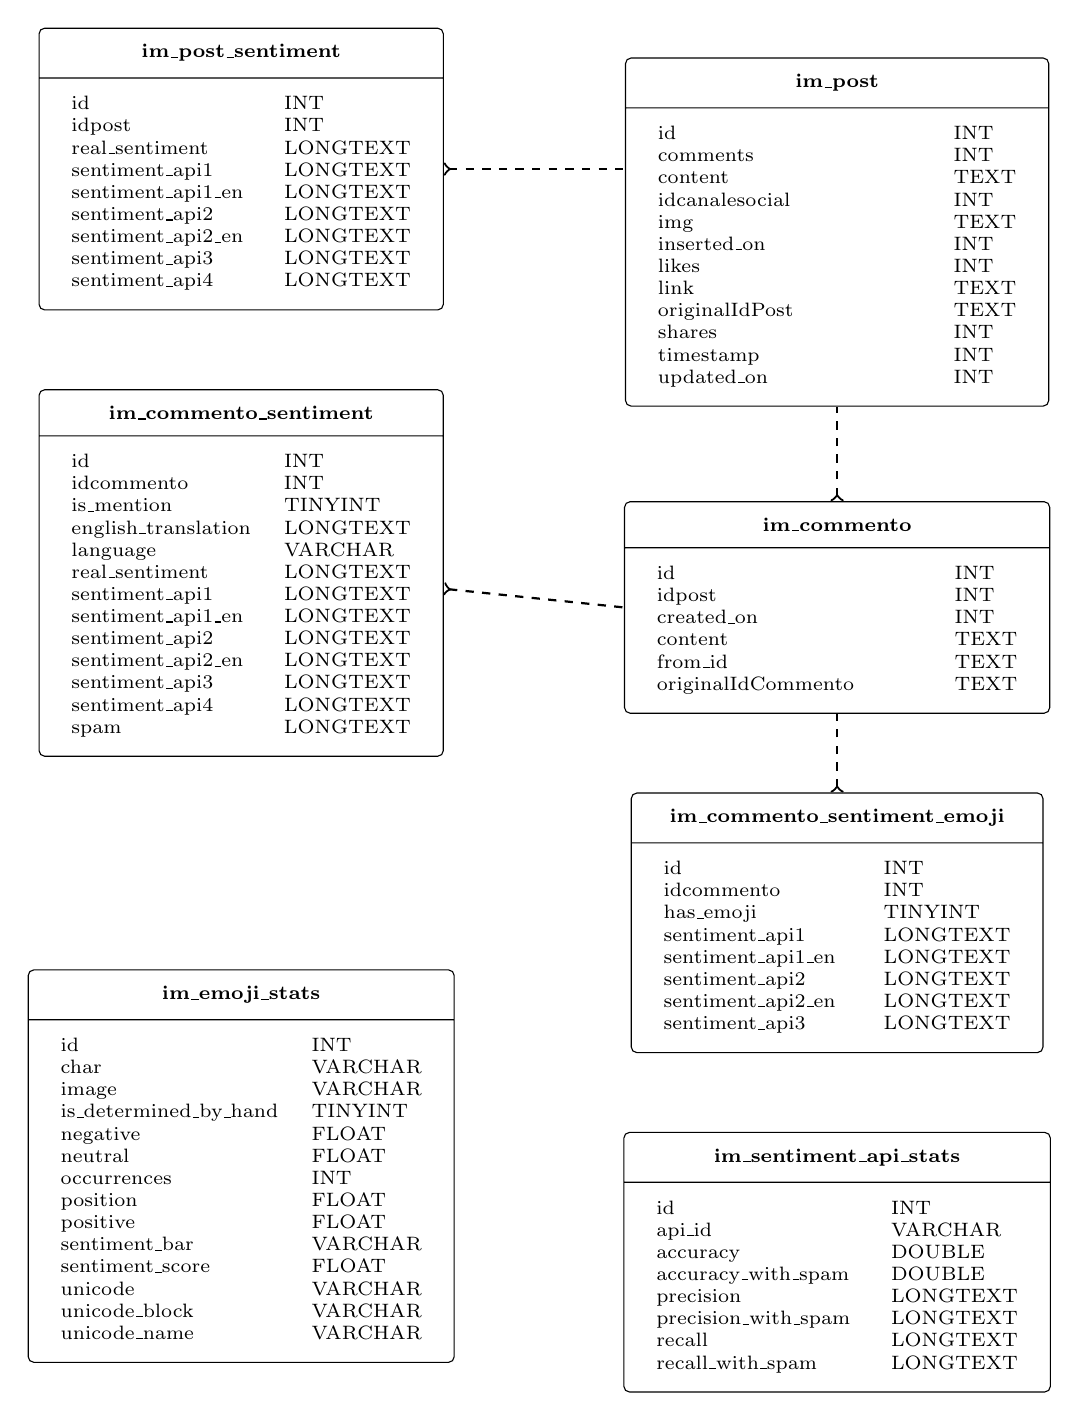
\begin{tikzpicture}[node distance=1cm]
\onehalfspacing

    \node (im-post) [table]{
        \textbf{im\_post}
        \nodepart{second}
            \tabular{ll} 
            id & INT \\ 
            comments & INT \\ 
            content & TEXT \\ 
            idcanalesocial & INT \\ 
            img & TEXT \\ 
            inserted\_on & INT \\ 
            likes & INT \\ 
            link & TEXT \\ 
            originalIdPost \ \ \ \ \ \ \ \ \ \ \ \ \ \ \ \ \ & TEXT \\
            shares & INT \\
            timestamp & INT \\
            updated\_on & INT \\                        
            \endtabular
    };

    \node (im-post-sentiment) [table, left=of im-post, yshift=0.8cm, xshift=-1.3cm]{
        \textbf{im\_post\_sentiment}
        \nodepart{second}
            \tabular{ll}                    
            id & INT \\
            idpost & INT \\
            real\_sentiment & LONGTEXT \\
            sentiment\_api1 & LONGTEXT \\
            sentiment\_api1\_en \ & LONGTEXT \\
            sentiment\_api2 & LONGTEXT \\
            sentiment\_api2\_en & LONGTEXT \\
            sentiment\_api3 & LONGTEXT \\
            sentiment\_api4 & LONGTEXT \\
            \endtabular
    };

    \node (im-commento) [table, below=of im-post,yshift=-0.2cm ]{
        \textbf{im\_commento}
        \nodepart{second}
            \tabular{ll}                    
            id & INT \\
            idpost & INT \\
            created\_on & INT \\
            content & TEXT \\
            from\_id & TEXT \\
            originalIdCommento \ \ \ \ \ \ \ \ \ & TEXT \\
            \endtabular
    };

    \node (im-commento-sentiment) [table, below=of im-post-sentiment]{
        \textbf{im\_commento\_sentiment}
        \nodepart{second}
            \tabular{ll}                    
            id & INT \\
            idcommento & INT \\
            is\_mention & TINYINT \\
            english\_translation & LONGTEXT \\
            language & VARCHAR \\
            real\_sentiment & LONGTEXT \\
            sentiment\_api1 & LONGTEXT \\
            sentiment\_api1\_en & LONGTEXT \\
            sentiment\_api2 & LONGTEXT \\
            sentiment\_api2\_en & LONGTEXT \\
            sentiment\_api3 & LONGTEXT \\
            sentiment\_api4 & LONGTEXT \\
            spam & LONGTEXT \\
            \endtabular
    };

    \node (im-commento-sentiment-emoji) [table, below=of im-commento]{
        \textbf{im\_commento\_sentiment\_emoji}
        \nodepart{second}
            \tabular{ll}                    
            id & INT \\
            idcommento & INT \\
            has\_emoji & TINYINT \\
            sentiment\_api1 & LONGTEXT \\
            sentiment\_api1\_en & LONGTEXT \\
            sentiment\_api2 & LONGTEXT \\
            sentiment\_api2\_en  \ \ & LONGTEXT \\
            sentiment\_api3 & LONGTEXT \\
            \endtabular
    };

    \node (im-sentiment-api-stats) [table, below=of im-commento-sentiment-emoji]{
        \textbf{im\_sentiment\_api\_stats}
        \nodepart{second}
            \tabular{ll}                    
            id & INT \\
            api\_id & VARCHAR \\
            accuracy & DOUBLE \\
            accuracy\_with\_spam & DOUBLE \\
            precision & LONGTEXT \\
            precision\_with\_spam \ & LONGTEXT \\
            recall & LONGTEXT \\
            recall\_with\_spam & LONGTEXT \\
            \endtabular
    };

    \node (im-emoji-stats) [table, below=of im-commento-sentiment, yshift=-1.7cm]{
        \textbf{im\_emoji\_stats}
        \nodepart{second}
            \tabular{ll}                    
            id & INT \\
            char & VARCHAR \\
            image & VARCHAR \\
            is\_determined\_by\_hand & TINYINT \\
            negative & FLOAT \\
            neutral & FLOAT \\
            occurrences & INT \\
            position & FLOAT \\
            positive & FLOAT \\
            sentiment\_bar & VARCHAR \\
            sentiment\_score & FLOAT \\
            unicode & VARCHAR \\
            unicode\_block & VARCHAR \\
            unicode\_name & VARCHAR \\
            \endtabular
    };

    \draw[line] (im-post-sentiment.east) -- ([yshift=0.8cm] im-post.west);
    \draw[line] (im-commento.north) -- (im-post.south);
    \draw[line] ([yshift=-0.2cm] im-commento-sentiment.east) -- (im-commento.west);
    \draw[line] ( im-commento-sentiment-emoji.north) |- (im-commento.south);
   
\end{tikzpicture}
  \caption{Database schema}
  \label{fig:db-schema}
\end{figure}